\documentclass[rnd]{extarticle}

\usepackage[utf8]{inputenc}
\usepackage{amsmath}
\usepackage{amsfonts}
\usepackage{amssymb}
\usepackage{graphicx}
\usepackage{blindtext}
\usepackage{csvsimple}
\usepackage{placeins}
\usepackage{hyperref}




\begin{document}  

	\title{Tweet Gendeer Classification}

	\author{AmirMohammad Azadi\\[0.2cm]{\small Advisors: Dr. Sauleh Etemadi, Hadi Sheikhi}}

	\date{July 2023}
	
	\maketitle

	\pagestyle{plain}
	
    \section{Repository}
		github repository: https://github.com/am-azadi/NLP_Project/tree/master
	
	\section{Source}
		Twitter doesn't save user genders. so using api we can not gather data with gender labels. so I used a preprovided dataset and download it form the below link:\\
        https://drive.google.com/uc?id=1rbQ5a95uyXl20TTECn3dS4dl42OTcmM_.\\
        there is a set of tweets with gender specified.\\

	\section{Data Format}
		Data is represented in four different directories. The data/raw path includes the raw tweets as a CSV file.\\
		The data/clean path includes a CSV file clean\_data that is the result of cleaning our raw data.\\
		
	\section{Preprocessing}
		After cleaning the data, we have a dataset that only have gender and text. we generate sentence and word tokenizations for each tweet and save it as json file in data/sentencebroken and data/wordbroken directories.\\
			
	\section{Statistics}
		
		\subsection{Data Count}
			
		\csvautotabular{../../stats/data_count.csv}

		
		\subsection{Sentence Count}
		
		\csvautotabular{../../stats/sentence_count.csv}


		\subsection{Word Count}
		
		\csvautotabular{../../stats/word_count.csv}

	
		\subsection{Unique Word Count}
	
		\csvautotabular{../../stats/unique_word_count.csv}
		
		
		\subsection{Common and Uncommon Unique Words}
		\begin{center}
			\csvautotabular{../../stats/count_common_and_uncommin_words.csv}
		\end{center}
	

        \subsection{Frequent Uncommon words}

		\csvautotabular{../../stats/frequent_uncommon_word.csv}
		
		
		\subsection{TF-IDF}
		\subsubsection{Male}
		\begin{center}
			\csvautotabular{../../stats/male_TF_IDF.csv}
		\end{center}
		\subsubsection{Female}
		\begin{center}
			\csvautotabular{../../stats/female_TF_IDF.csv}
		\end{center}

		
		\subsection{Top Unique Words}
		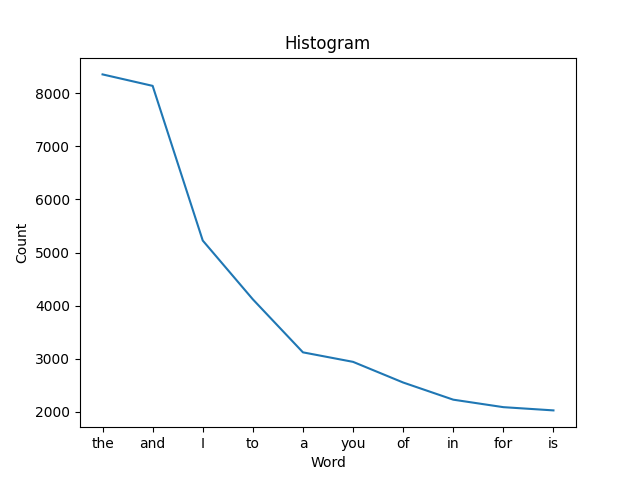
\includegraphics[width=1\textwidth]{../../stats/top_unique_words.png}
	
	
\end{document}